\documentclass[letterpaper,10pt]{article}

\usepackage{enumitem}
\usepackage{titling}
\usepackage{listings}
\usepackage{url}
\usepackage{hyperref}
\usepackage{setspace}
\usepackage{subfig}
\usepackage{sectsty}
\usepackage{pdfpages}
\usepackage{colortbl}
\usepackage{multirow}
\usepackage{multicol}
\usepackage{relsize}
\usepackage{amsmath}
\usepackage{wasysym}
\usepackage{fancyvrb}
\usepackage[yyyymmdd]{datetime}
\usepackage{amsmath,amssymb,amsthm,graphicx,xspace}
\usepackage[titlenotnumbered,noend,noline]{algorithm2e}
\usepackage[compact]{titlesec}
\usepackage{XCharter}
\usepackage[T1]{fontenc}
\usepackage[scaled]{beramono}
\usepackage[normalem]{ulem}
\usepackage{booktabs}
\usepackage{tikz}
\usetikzlibrary{arrows,automata,shapes,trees,matrix,chains,scopes,positioning,calc}
\tikzstyle{block} = [rectangle, draw, fill=blue!20,
text width=2.5em, text centered, rounded corners, minimum height=2em]
\tikzstyle{bw} = [rectangle, draw, fill=blue!20,
text width=4em, text centered, rounded corners, minimum height=2em]

\definecolor{namerow}{cmyk}{.40,.40,.40,.40}
\definecolor{namecol}{cmyk}{.40,.40,.40,.40}
\renewcommand{\dateseparator}{-}

\let\LaTeXtitle\title
\renewcommand{\title}[1]{\LaTeXtitle{\textsf{#1}}}

\lstset{basicstyle=\footnotesize\ttfamily,breaklines=true}

\newcommand{\handout}[5]{
	\noindent
	\begin{center}
		\framebox{
			\vbox{
				\hbox to 5.78in { {\bf ECE 350: Real-Time Operating Systems } \hfill #2 }
				\vspace{4mm}
				\hbox to 5.78in { {\Large \hfill #4  \hfill} }
				\vspace{2mm}
				\hbox to 5.78in { {\em #3 \hfill \today} }
			}
		}
	\end{center}
	\vspace*{4mm}
}

\newcommand{\lecture}[3]{\handout{#1}{#2}{#3}{Lecture#1}}
\newcommand{\tuple}[1]{\ensuremath{\left\langle #1 \right\rangle}\xspace}

\newcommand{\Rplus}{\protect\hspace{-.1em}\protect\raisebox{.35ex}{\smaller{\smaller\textbf{+}}}}
\newcommand{\Cpp}{\mbox{C\Rplus\Rplus}\xspace}


\addtolength{\oddsidemargin}{-1.000in}
\addtolength{\evensidemargin}{-0.500in}
\addtolength{\textwidth}{2.0in}
\addtolength{\topmargin}{-1.000in}
\addtolength{\textheight}{1.75in}
\addtolength{\parskip}{\baselineskip}
\setlength{\parindent}{0in}
\renewcommand{\baselinestretch}{1.5}
\newcommand{\term}{Spring 2023}
\newcommand{\termnumeric}{1235}

\singlespace


\begin{document}

\lecture{ 19 --- Input/Output Devices \& Drivers}{\term}{Jeff Zarnett}

\section*{Input/Output Devices}
Though the computer's name and typical use kind of suggests the purpose of the machine is computation, input/output is just as important to the usefulness of a computer. A computer that takes no inputs and produces no outputs is, presumably, not very useful\footnote{Schr\"odinger's computer: did the program actually run if there was no output to observe?}. I/O is, unfortunately, a messy business. Whereas there are only a small number of CPU types your typical desktop OS might run (and the AMD and Intel processors, for example, can execute the same binary code), there are uncountably many I/O devices in the world. And they're all different. Keyboards, hard drives, printers, and headsets are all I/O devices, but they serve very different purposes and work in different ways. This diagram shows the dramatic differences in speed between various devices of a typical PC:

\begin{center}
	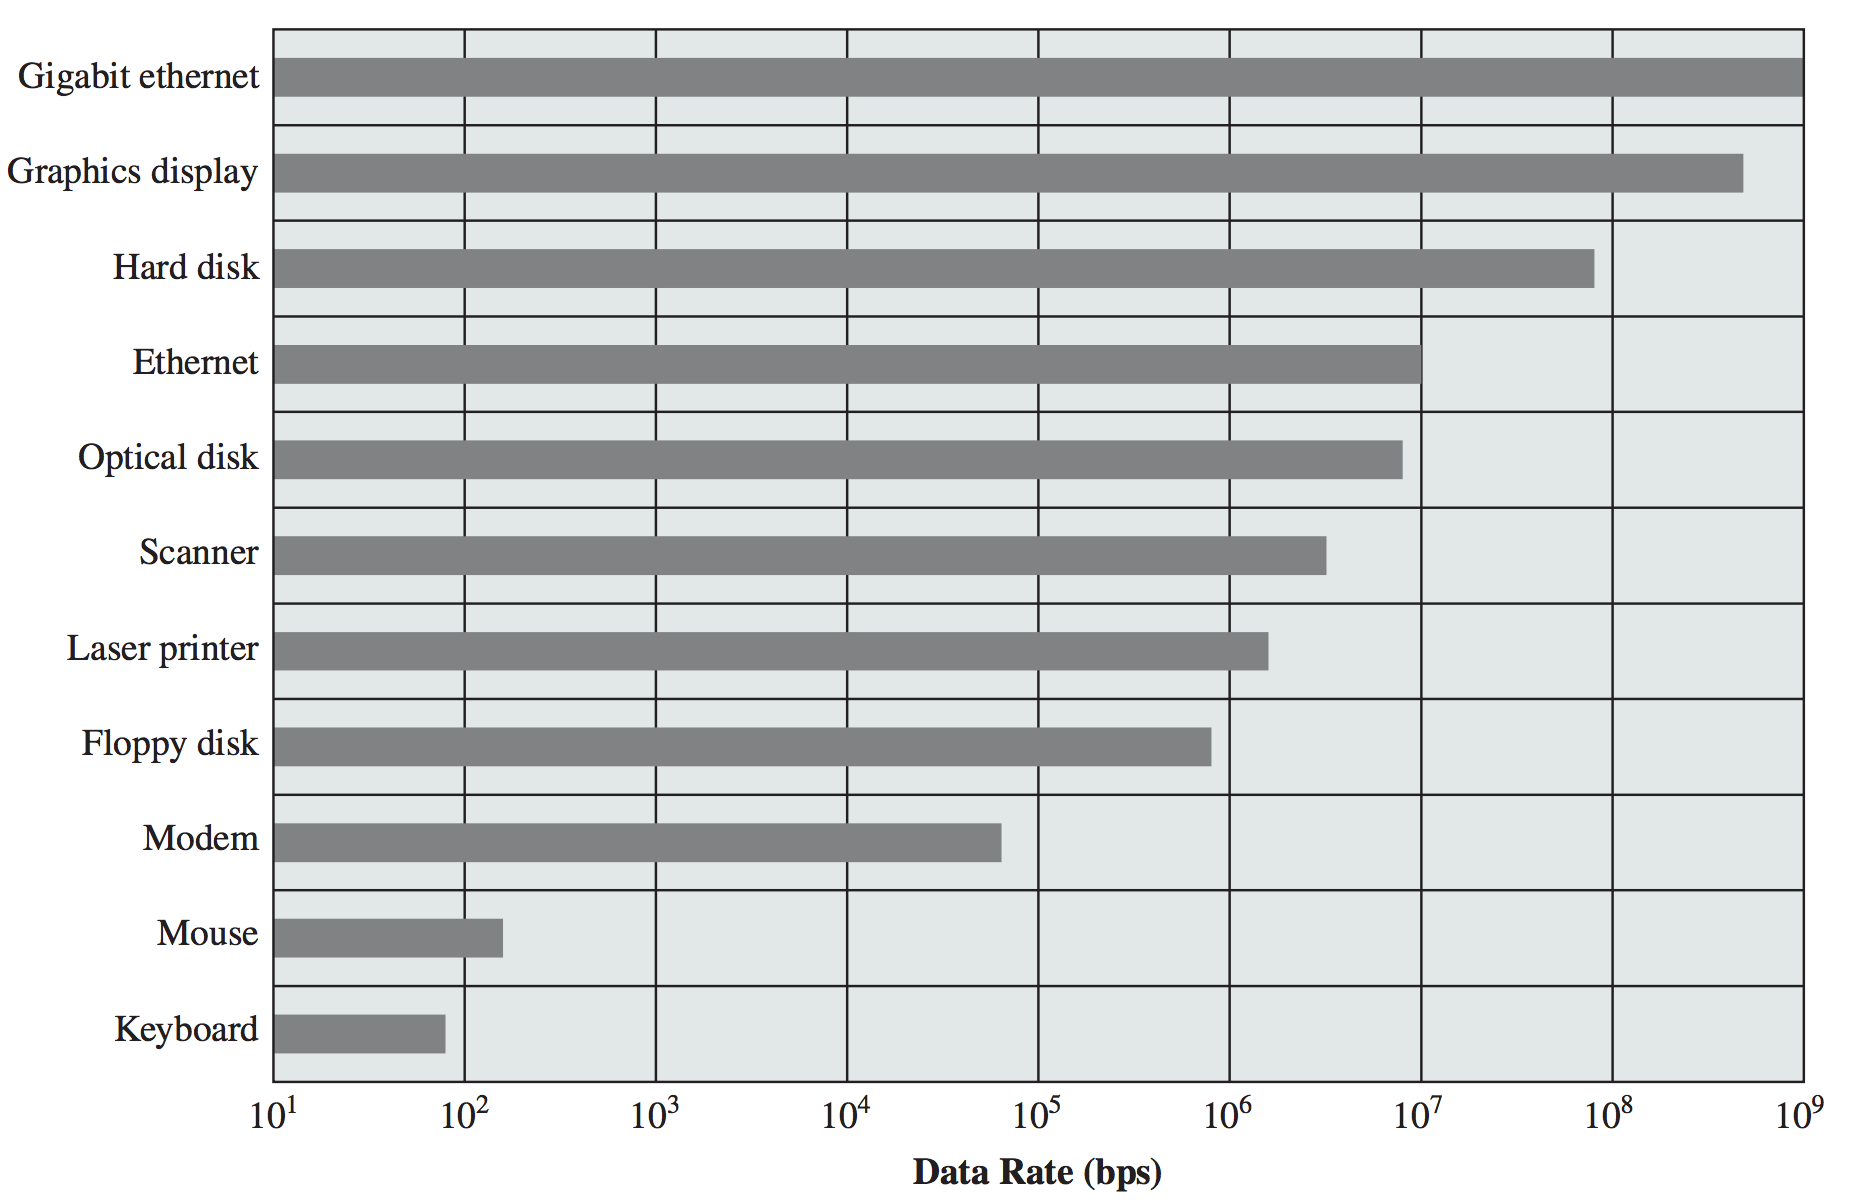
\includegraphics[width=0.75\textwidth]{images/io-device-rates.png}\\
	Typical I/O Device Data Rates~\cite{osi}.
\end{center}

We might like to think that USB has taken away some of the complexity, but that's just the way a device connects to the computer; managing the device itself is still as complicated as ever. All of the examples just listed in the previous paragraph can be connected via USB (Universal Serial Bus). 

Disk I/O, when discussing magnetic hard disks, has a huge impact on system performance that it will receive its own discussion. But first, a little discussion about I/O in general.

We will not be spending any time talking about the specifics of the hardware (though it might be helpful to review that information on your own). For I/O the key parts are the bus (and a modern PC has several, including the PCIe bus, USB, etc.) and a controller (electronics to operate the hardware port, bus, device...). After that there will be a system or protocol for how the devices will communicate, whether it is polling, interrupts, or DMA (Direct Memory Access) as discussed earlier. With that out of the way, let us examine devices at a higher level.

\subsection*{Application I/O Interface}

Ideally, when a general-purpose operating system is written, it will accept new devices being added to the system without editing/reinstalling/recompiling the code. Your experience with object oriented programming gives you some familiarity with the solution of how we should accomplish this goal. We want to abstract away the details of the hardware, to the extent we can, and provide a uniform \textit{interface} to interact with. 

In the very early days of operating systems, the hardware the computer shipped with was all the hardware it ever supported. If the vendor came out with a new module, they would have a new operating system update to introduce support for that device. This got to be unmanageable in the era of the IBM PC because anybody could create hardware and attach it via a standard interface. Relying on IBM or Microsoft or whoever your OS vendor was to implement support for a random piece of hardware was not realistic.

Operating system developers thought they were very clever. They realized that they could shift the work to the hardware developers through a concept called \textit{device drivers}. The device driver plugs in to the operating system through a standard interface and tells the operating system a bit about the hardware and translates commands from the operating system to hardware instructions. Where this fell apart was the fact that hardware developers often made extremely poor drivers (whether this was due to inability or lack of caring is not clear).

The problem was exacerbated by a Windows design decision that device drivers would run in the system at the same protection level as the kernel. Some other operating systems have user-mode drivers, where possible (in Mac OS X and Linux systems, for example, there is the ability to have file system drivers in user space through a program called FUSE) or at an intermediate level between that of user space and the kernel. In any event, in Windows, if a device driver is unhappy with the current state of the system, contains a programming error, or encounters a situation it cannot handle, the driver can invoke a system call that brings up everyone's favourite feature: the Blue Screen of Death (BSOD).

Microsoft, rightly or wrongly, was blamed for a lot of those blue screens of death. They took two approaches to remedy this problem. One was to write and include in Windows a lot more device drivers. The other was to introduce the static driver verifier, a complex piece of static analysis software used to test, at compile/build time, whether the driver will behave badly. Passing this test is required to get a sticker of approval from Microsoft to put on the box. So, the battle rages on about who is responsible for writing the drivers, unfortunately.

Device drivers, when they exist, connect into the kernel's I/O subsystem to mediate between the kernel's I/O subsystem and the hardware device controller. See the diagram:

\begin{center}
	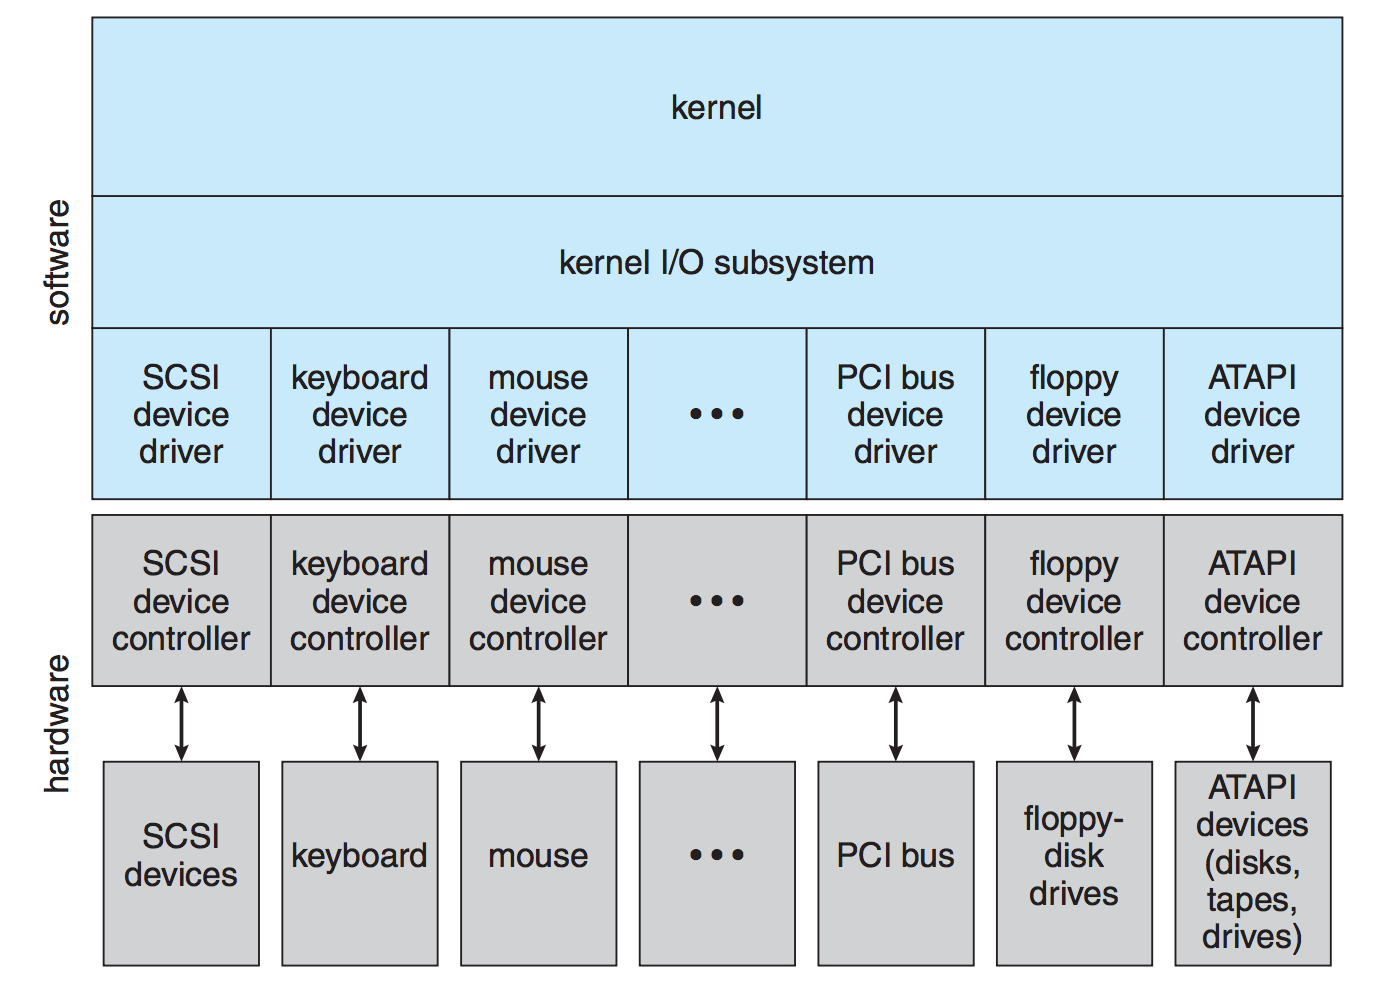
\includegraphics[width=0.65\textwidth]{images/kernel-io-structure.png}\\
	Kernel I/O structure, showing the placement of device drivers~\cite{osc}.
\end{center}

Abstracting away details of the hardware makes the job of the operating system developer easier: the interface provides a standard way of interacting with the hardware device. Part of the difficulty is that devices can vary on numerous dimensions, as we can see through a few examples from~\cite{osc}:

\begin{itemize}
\item \textbf{Data transfer mode}. A device may operate on a character level (transfer one character at a time) like a keyboard, or may operate on a block (group of bytes) all at once, such as a disk operating on a 4~KB block.
\item \textbf{Access method}. A device may allow only sequential access (that is, reading only the next element or piece of data or writing to the next location) such as a modem, or it could allow random access (reading from or writing to any point) as in a CD (compact disc). 
\item \textbf{Transfer schedule}. The schedule may be synchronous (transferring data with predictable response times) as in the case of reading from tape, or asynchronous (with unpredictable response times), such as awaiting a response that will come over the network.
\item \textbf{Dedication}. A device may be shareable (allows multiple concurrent threads) such as the speakers, or dedicated (allowing only one thread to use it at a time), such as a printer.
\item \textbf{Device Speed}. Recall the diagram from earlier showing the dramatic differences in transfer speeds.
\item \textbf{Transfer Direction}. Some devices are input only (such as a temperature sensor), other devices are output only (speakers), and some devices are capable of both (hard disk).
\end{itemize}

We would like to, as much as possible, keep the details above from the operating system, though devices will typically be grouped into a few categories so appropriate system calls can be issued. If a device is block-oriented, the OS should be issuing block read and write commands, not trying to do it one character at a time.

Operating systems also usually have an \textit{escape} system call that allows passing of a command directly from an application or the kernel to a device driver. This allows us to issue commands to a device that the OS designers have not thought of and created system calls for. The UNIX system call for this is \texttt{ioctl} (``I/O Control'') and it takes three parameters: a file descriptor indicating the hardware device (everything in UNIX is a file, remember), the command number (an integer), and a pointer to an arbitrary data structure (presumably \texttt{void*}) that has any necessary control information and data~\cite{osc}.

\subsection*{Block and Character I/O}

The block device interface is used for block devices such as hard disk drives. Any device will support \texttt{read} and \texttt{write} commands, and if it is a random-access device, it will have a \texttt{seek} command to jump to a specific block. An application usually accesses the hard disk through the file system, but going even one level lower, the OS can work on the hard drive using these two/three commands without being concerned with how that command is actually transmitted to the physical hardware.

We can abstract things a little bit further, from the perspective of the application developer, by having a memory-mapped file. Then, rather than using the block oriented operations directly, the application just writes to and reads from ``memory'' and the OS handles the behind-the-scene coordination to make writes go out to the correct block and read from the correct block.

A character-oriented device is something like the keyboard; the system calls are \texttt{get} and \texttt{put}. Libraries and other structures may exist to work on a whole line at a time (compare to, for example, the Java constructs for reading and writing files: the default streams are one character at a time, but if you want anything other than terrible performance, use a buffered reader which can read a whole line). This is a good match for input devices that produce data in small amounts and at unpredictable times, and perhaps for printers and sound output which operate naturally on a linear stream of bytes~\cite{osc}.


\subsection*{Buffering}

Regardless of whether a device is block- or character-oriented, the operating system can improve its performance through the use of buffering. As you may have experienced with Java, the use of a buffer speeds things up quite a lot. A buffer is nothing more than an area of memory that stores data being transferred, whether it is from memory to a device, device to memory, or device to device. 

A buffer is a good way to deal with a speed mismatch between devices. Users type very slowly, from the perspective of the computer, and it would be awfully inefficient to ask the disk, a block oriented device, to update itself on every single character. It is much better if we wait until we have some certain amount of data (e.g., a whole line or whole block or full buffer, whichever it is) and then write this out to disk all at once. 

The write is, however, not instantaneous and in the meantime, the user can still keep typing. Thus, to solve this, the typical solution is \textit{double buffering}, that is, two buffers. While buffer one is being emptied, buffer two receives any incoming keystrokes. Double buffering decouples the producer and consumer of data, helping to overcome speed differences between the two~\cite{osc}.


\subsection*{Network Devices}

Network devices are fundamentally different from those that are directly attached to the system. Thus, the \texttt{read}, \texttt{write}, and \texttt{seek} routines are not really appropriate. The model we are most familiar with from UNIX and Windows is that of \textit{sockets}.
To support servers with multiple clients, the socket interface has a function \texttt{select}, that manages a set of sockets. Invoking this function returns information about what sockets have a packet waiting to be received and which are available for sending a packet. Proper use of \texttt{select} eliminates polling and busy-waiting in a situation where delays are unpredictable (which is always the case with the network).


\subsection*{Spooling and Reservations}
A \textit{spool} is a buffer for a device, like a printer, that can serve only one job at a time. Unlike disk, where it might read for $P_{1}$ now and then write for $P_{2}$ immediately afterwards, a printer needs to finish a whole print job before it starts the next. Printing is the most obvious example, but it is by no means the only one. The operating system centralizes all communication to the printer and runs it through the spooling system. 

\subsection*{I/O Protection}
Recall from much earlier the idea of kernel mode and user mode instructions; some processor instructions are restricted such that only the OS can issue them (in kernel mode), otherwise it is an error (illegal instruction). We want all user accesses to I/O to be mediated through the operating system, so the OS can check to see if the request is valid. If it is, allow it to proceed; otherwise terminate the process with an error. This helps minimize errors and problems where people do bad things like cancel another process's request so theirs can go first. Our typical tradeoff: increased safety in exchange for reduced performance.

In certain circumstances, for performance reasons, we might want to allow direct access. In the case of a game, for example, we want to allow the game to work directly on the graphics card's memory (despite the fact that it is an I/O device). Mediating every access through the kernel would result in unacceptably poor performance (which is to say, the other team would totally call us noobs). So a section of graphics memory, corresponding to a particular window on the screen, will be locked by the kernel to be accessible by the game's process~\cite{osc}.

\subsection*{Kernel I/O Data Structures}
The kernel must, as is rather obvious, keep track of what I/O devices are in use by which processes and the general state of the I/O device (``PC Load Letter''). The diagram below gives some indication of what the UNIX kernel structures are like for open files:

\begin{center}
	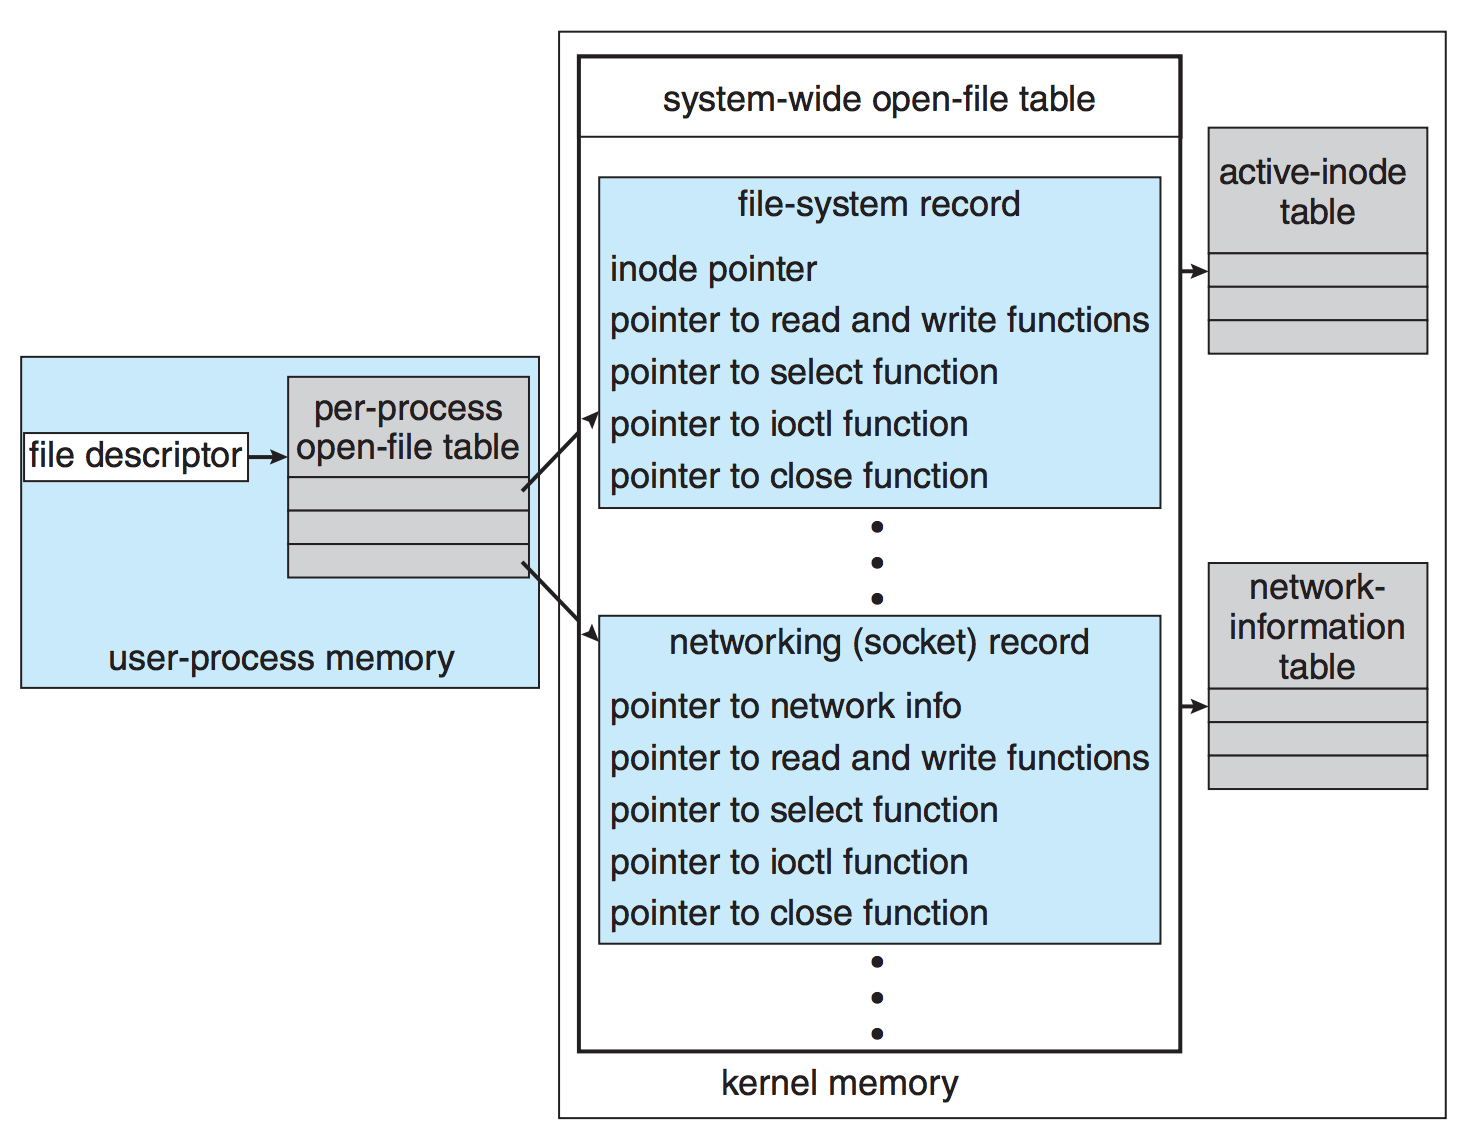
\includegraphics[width=0.7\textwidth]{images/unix-io-kernel.png}\\
	The UNIX structures to manage I/O~\cite{osc}.
\end{center}

\subsection*{I/O Scheduling}

As a final note, we sometimes want to schedule I/O requests in some order other than First-Come, First-Served. A simple analogy: Imagine you need to go to the grocery store, the dry cleaners, and the bank. The bank is located 1~km to the west of your current location, and the grocery store is 3~km west. The dry cleaners is in the same plaza as the grocery store. It is obvious that it would be fine to go to the bank, then the dry cleaners, then the grocery store, but not to go to the dry cleaners, then the bank, then the grocery store. The unnecessary back-and-forth wastes time and energy (whether walking or fuel depends on your mode of transportation).

Clearly, the operating system will want to do something similar with I/O requests. It will maintain a structure of requests and can then re-arrange them to be accomplished most efficiently. The literature sometimes refers to this as a queue but... is it really a queue when it does not exhibit the first-in, first-out behaviour\footnote{But I'm kind of strict about my use of grammar and language. Things like ``10 items or less'' signs bother me, because I know it should be ``10 items or \textbf{fewer}''. For those who are fans of \textit{Game of Thrones}, it will probably not surprise you that I like Stannis Baratheon.}? This will, naturally, have some limits: requests should presumably get scheduled before too much time has elapsed even if it would be ``inconvenient''. It might also take priority into account, dealing with the I/O requests of a high priority process even if they are not particularly nearby to other requests. 

In particular, this is important when examining hard disk drive operation. And that will therefore be the next subject we will consider.

\section*{Transforming I/O Requests to Hardware Operations}

In the previous section we discussed the idea of taking a command like \texttt{read} and said it is the job of the device driver to translate this command into a hardware operation. Reading from the file system on disk, for example, requires a few steps. If I want to open a file like \texttt{example.txt}, the file system (not yet discussed) will associate this file with some information about where on the disk this is (a set of disk blocks representing the file). Then, to read the file, \texttt{read} commands can be issued to get those blocks into memory so I can edit it with \texttt{vi}.

The diagram below shows the life cycle of an I/O request:

\begin{center}
	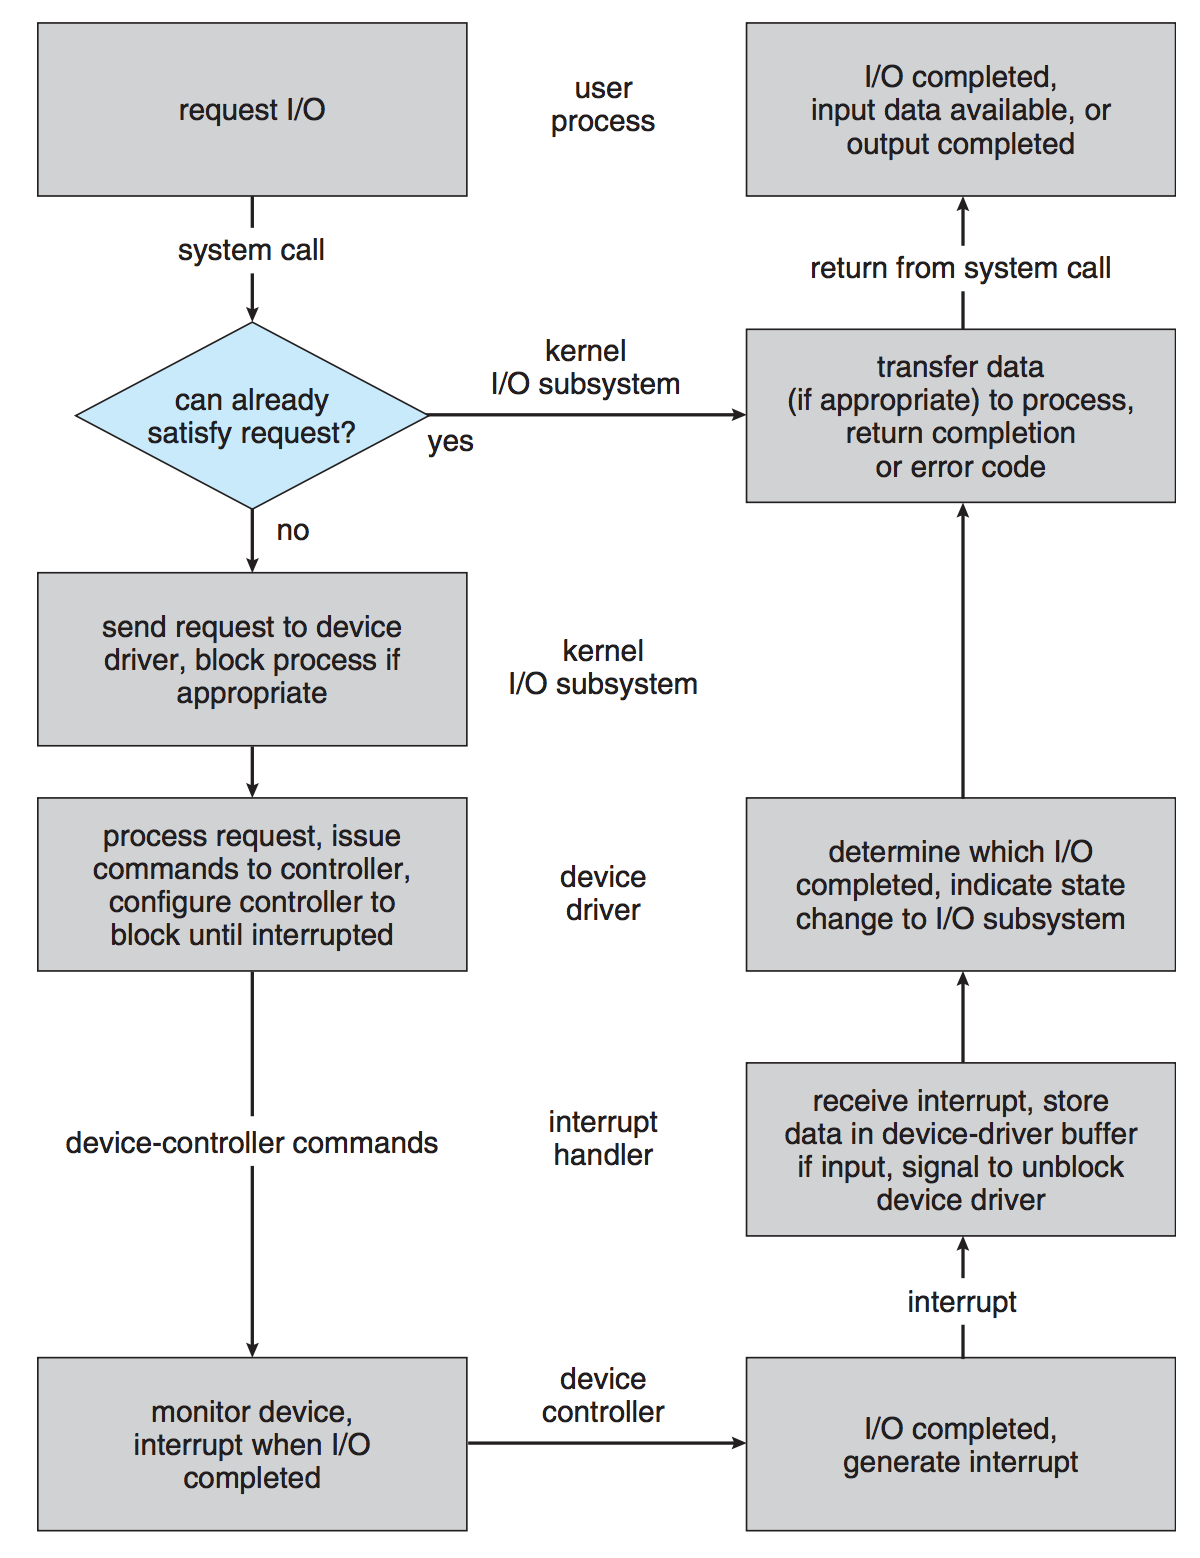
\includegraphics[width=0.65\textwidth]{images/io-lifecycle.png}\\
	The life cycle of an I/O request~\cite{osc}.
\end{center}

In general, the life cycle follows some ten steps from start to finish~\cite{osc}:

\begin{enumerate}
	\item A process issues a \texttt{read} command (assume the file is already open).
	\item The system call routine checks the parameters for correctness. If the data is in a cache or buffer, return it straight away.
	\item Otherwise, the process is blocked waiting for the device and the I/O request is scheduled. When the operation is to take place, the I/O subsystem tells the device driver.
	\item The device driver allocates a buffer to receive the data. The device is signalled to perform the I/O (usually by writing into device-control registers or sending a signal on a bus).
	\item The device controller operates the hardware to do the work.
	\item The driver may poll for status, await the interrupt when finished, or for the DMA controller to signal it is finished.
	\item The interrupt handler receives the interrupt and stores the data; it then signals the device driver to indicate the operation is done.
	\item The device driver identifies what operation has just finished, determines the status, and tells the I/O subsystem it is done.
	\item The kernel transfers the data (or error code or whatever) to the address space of the requesting process, and unblocks that process.
	\item When the scheduler chooses that process, it resumes execution.
\end{enumerate}

\bibliographystyle{alphaurl}
\bibliography{350}


\end{document}